\chapter{Efficiënte zoekbomen}

\section{Inleiding}
\begin{itemize}
    \item Uitvoeringstijd van operaties (zoeken, toevoegen, verwijderen) op een binaire zoekboom met hoogte $h$ is $O(h)$.
    \item De hoogte $h$ is afhankelijk van de toevoegvolgorde:
    \begin{itemize}
        \item In het slechtste geval bekomt men een gelinkte lijst, zodat $h = O(n)$.
        \item Als elke toevoegvolgorde even waarschijnlijk is, dan is de verwachtingswaarde voor de hoogte $h = O(\lg n)$ met $n$ het aantal gegevens.
        \begin{itemize}
            \alert Geen realistische veronderstelling.
        \end{itemize}
    \end{itemize}
    \item \underline{Drie manieren} om de efficiëntie van zoekbomen te verbeteren:
    \begin{enumerate}
        \item \textbf{Elke operatie steeds efficiënt maken.}
        \begin{enumerate}
            \item AVL-bomen.
            \begin{itemize}
                \item Hoogteverschil $\Delta h$ van de twee deelbomen van elke knoop is kleiner of gelijk aan 1.
                \item $\Delta h$ wordt opgeslagen in de knoop zelf.
                \begin{figure}[ht]
                    \centering
                    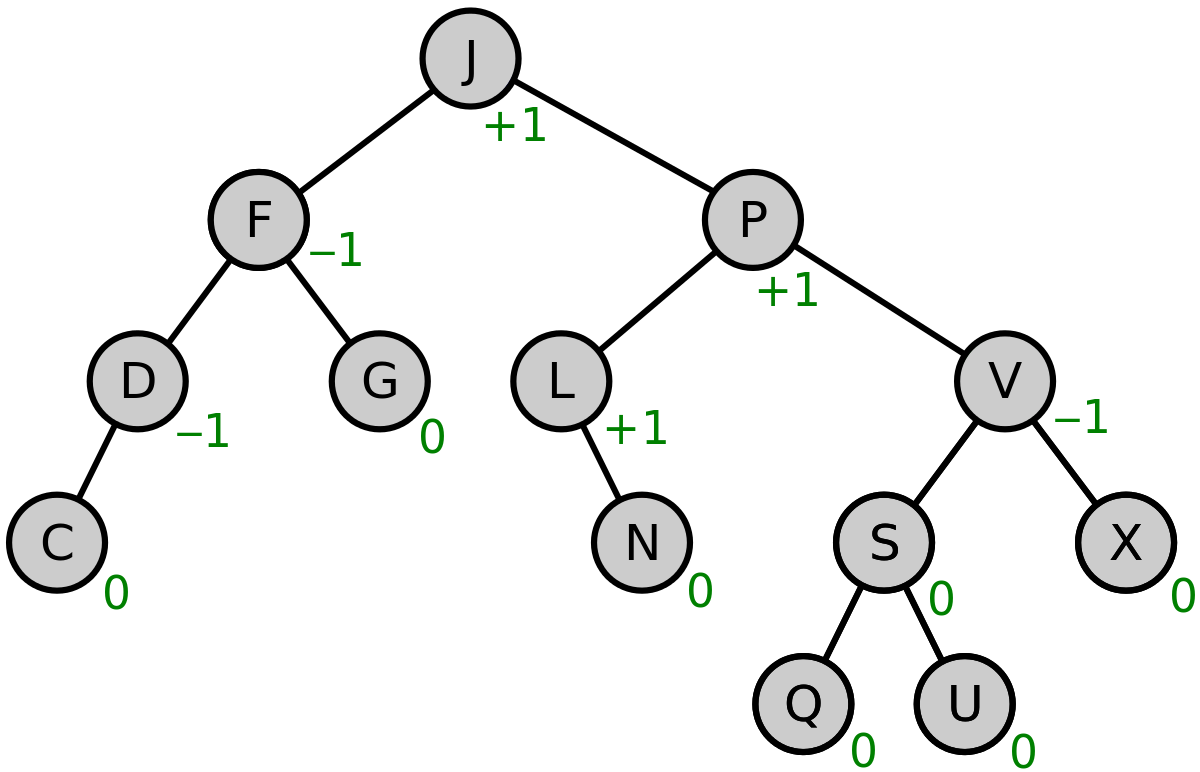
\includegraphics[width=0.5\textwidth]{AVL-tree}
                    \caption{Een AVL-boom. De groene cijfers stellen de hoogteverschillen voor van de twee deelbomen voor elke knoop.}
                    \label{fig:AVL-tree}
                \end{figure}
            \end{itemize}
            \item 2-3-bomen.
            \begin{itemize}
                \item Elke knoop heeft 2 of 3 kinderen.
                \item Elk blad heeft dezelfde diepte.
                \item Bij toevoegen of verwijderen wordt het ideale evenwicht behouden door het aantal kinderen van de knopen te manipuleren.
            \end{itemize}
            \item 2-3-4-bomen.
            \begin{itemize}
                \item Eenvoudiger dan 2-3-bomen om te implementeren.
            \end{itemize}
            \item Rood-zwarte bomen (sectie \ref{sec:rood-zwarte bomen}).
        \end{enumerate}

        \item \textbf{Elke reeks operaties steeds efficiënt maken.}
        \begin{enumerate}
            \item Splaybomen (sectie \ref{sec:splaybomen}).
            \begin{itemize}
                \item De vorm van de boom wordt meermaals aangepast.
                \item Elke reeks opeenvolgende operaties is gegarandeerd efficiënt.
                \item Een individuele operatie kan wel traag uitvallen.
                \item \textit{Geamortiseerd} is de performantie per operatie goed.
            \end{itemize}
        \end{enumerate}

        \item \textbf{De gemiddelde efficiëntie onafhankelijk maken van de operatievolgorde.}
        \begin{enumerate}
            \item Gerandomiseerde zoekbomen (sectie \ref{sec:gerandomiseerde-zoekbomen}).
            \begin{itemize}
                \item Gebruik van een random generator.
                \item De boom is random, onafhankelijk van de toevoeg- en verwijdervolgorde.
                \item Verwachtingswaarde van de hoogte $h$ wordt dan $O(\lg n)$.
            \end{itemize}
        \end{enumerate}
    \end{enumerate}
\end{itemize}

\section{Rood-zwarte bomen}
\subsection{Definitie en eigenschappen}
\begin{figure}[ht]
    \centering
    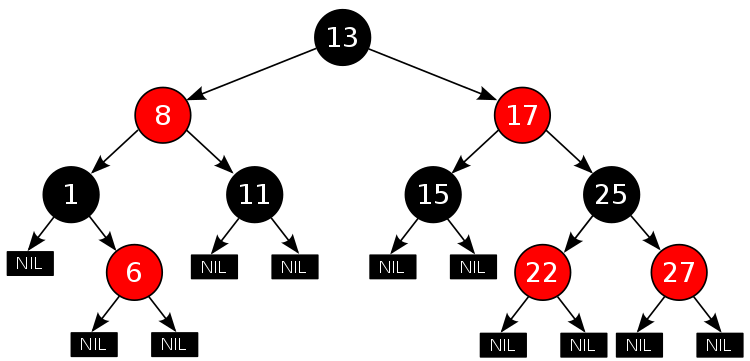
\includegraphics[width=\textwidth]{red-black-tree}
    \caption{Een rood-zwarte boom. De \texttt{NIL} knopen stellen virtuele knopen voor.}
    \label{fig:red-black-tree}
\end{figure}
\label{sec:rood-zwarte bomen}
\begin{itemize}
    \item \textbf{Definitie:}
    \begin{itemize}
        \item Een binaire zoekboom.
        \item Elke knoop is rood of zwart gekleurd.
        \item Elke virtuele knoop is zwart. Een virtuele knoop is een knoop die geen waarde heeft, maar wel een kleur. Deze vervangen de nullwijzers.
        \item Een rode knoop heeft steeds twee zwarte kinderen
        \item Elke mogelijke weg vanuit een knoop naar een virtuele knoop bevat evenveel zwarte knopen. Dit aantal wordt de \textit{zwarte hoogte} genoemd
        \item De wortel is zwart.
    \end{itemize}
    \item \textbf{Eigenschappen:}
    \begin{itemize}
        \item Een deelboom met wortel $w$ en zwarte hoogte $z$ heeft tenminste $2^z - 1$ inwendige knopen.
        \item De hoogte van een rood-zwarte boom met $n$ knopen is steeds $O(\lg n)$.
        \begin{itemize}
            \item Er zijn nooit twee opeenvolgende rode knopen op elke weg vanuit een knoop naar een virtuele knoop $\rightarrow z \geq h/2$.
            \item Substitutie in de eerste eigenschap geeft:
            \begin{align*}
                n &\geq 2^z - 1 \geq 2^{h/2} - 1 \\
                \rightarrow h & \leq 2\lg(n + 1)
            \end{align*}
        \end{itemize}
    \end{itemize}

\end{itemize}
\subsection{Zoeken}
\begin{itemize}
    \item De kleur speelt geen rol, zodat de rood-zwarte boom een gewone binaire zoekboom wordt.
    \item De hoogte van een rood-zwarte boom is wel gegerandeerd $O(\lg n)$.
    \item Zoeken naar een willekeurige sleutel is dus $O(\lg n)$.
\end{itemize}

\subsection{Toevoegen en verwijderen}
\begin{itemize}
    \item Element toevoegen of verwijderen, zonder rekening te houden met de kleur, is ook $O(\lg n)$.
    \alert Geen garantie dat deze gewijzigde boom nog rood-zwart zal zijn.
    \item Twee manieren om toe te voegen:
    \begin{enumerate}
        \item \textbf{Bottom-up:} 
        \begin{itemize}
            \item Voeg knoop toe zonder rekening te houden met de kleur.
            \item Herstel de rood-zwarte boom, te beginnen bij de nieuwe knoop, en desnoods tot bij de wortel.
        \end{itemize}
        \item \textbf{Top-down:} 
        \begin{itemize}
            \item Pas de boom aan langs de dalende zoekweg.
            \good Efficiënter dan bottom-down aangezien er geen ouderwijzers of een stapel nodig is.
        \end{itemize}
    \end{enumerate}
\end{itemize}

\subsection{Rotaties}
\begin{figure}[ht]
    \centering
    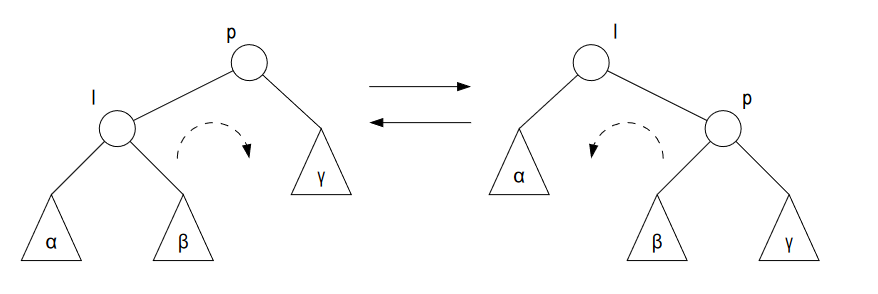
\includegraphics[width=0.5\textwidth]{rotations}
    \caption{Rotaties}
    \label{fig:rotations}
\end{figure}
\begin{itemize}
    \item Wijzigen de vorm van de boom, maar behouden de inorder volgorde van de sleutels.
    \item Moet enkel pointers aanpassen, en is dus $O(1)$.
    \item \textbf{Rechtste rotatie} van een ouder $p$ en zijn linkerkind $l$:
    \begin{itemize}
        \item Het rechterkind van $l$ wordt het linkerkind van $p$.
        \item De ouder van $p$ wordt de ouder van $l$.
        \item $p$ wordt het rechterkind van $l$. 
    \end{itemize}
    \item \textbf{Linkse rotatie} van een ouder $p$ en zijn rechterkind $r$:
    \begin{itemize}
        \item Het linkerkind van $r$ wordt het rechterkind van $p$.
        \item De ouder van $r$ wordt de ouder van $p$.
        \item $p$ wordt het linkerkind van $l$. 
    \end{itemize}
\end{itemize}

\subsection{Bottom-up rood-zwarte bomen}
\subsubsection{Toevoegen}



\subsubsection{Verwijderen}

\subsection{Top-down rood-zwarte bomen}
\subsubsection{Toevoegen}
\begin{itemize}
    \item De knoop wordt eerst op de gewone manier toegevoegd.
    \item Welke kleur geven we die knoop?
    \begin{itemize}
        \item \textbf{Zwart:} dit kan de zwarte hoogte van veel knopen ontregelen.
        \item \textbf{Rood:} dit mag enkel als de ouder zwart is.
        \item Kies voor rood omdat zwarte hoogte moeilijker te herstellen valt.
    \end{itemize}
    \item Als de ouder zwart is, dan is toevoegen gelukt.
    \item Als de ouder rood is wordt deze storing verwijderd door rotaties en kleurwijzigingen door te voeren.
    \item Vaststellingen:
    \begin{itemize}
        \item De ouder $p$ van de nieuwe knoop $c$ is rood.
        \item De ouder $g$ van $p$, is zwart.
    \end{itemize}
    \item Er zijn zes mogelijke gevallen, die twee groepen van drie vormen, naar gelang dat $p$ een linker- of rechterkind is van $g$. 
    \item We onderstellen dat $p$ een linkerkind is van $g$. 
    \begin{enumerate}
        \item \textbf{De broer $b$ van $p$ is rood.}
        \begin{figure}[ht]
            \centering
            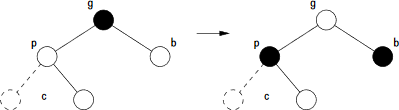
\includegraphics[width=0.5\textwidth]{rbt_bottomup_case1}
            \caption{Rode broer.}
            \label{fig:rbt_bottomup_case1}
        \end{figure}
        \begin{itemize}
            \item Maak $p$ en $b$ zwart.
            \item Maak $g$ rood.
            \item Als $g$ een zwarte ouder heeft, is het probleem opgelost.
            \item Als $g$ een rode ouder heeft, zijn er opnieuw twee opeenvolgende rode knopen.
            \item Het probleem wordt opgeschoven in de richting van de wortel.
        \end{itemize}
        \item \textbf{De broer $p$ van $p$ is zwart.}
        \begin{enumerate}
            \item \textbf{Knoop $c$ is een linkerkind van $p$.}
            \begin{figure}[ht]
                \centering
                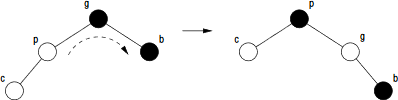
\includegraphics[width=0.5\textwidth]{rbt_bottomup_case2}
                \caption{Rode broer.}
                \label{fig:rbt_bottomup_case1}
            \end{figure}
            \begin{itemize}
                \item Roteer $p$ en $g$ naar rechts. 
                \item Maak $p$ zwart.
                \item Maak $g$ rood.
            \end{itemize}
            \item \textbf{Knoop $c$ is een rechterkind van $p$.}
            \begin{figure}[ht]
                \centering
                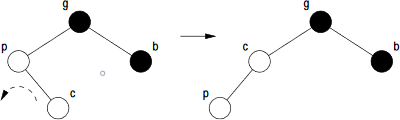
\includegraphics[width=0.5\textwidth]{rbt_bottomup_case3}
                \caption{Rode broer.}
                \label{fig:rbt_bottomup_case1}
            \end{figure}
            \begin{itemize}
                \item Roteer $p$ en $c$ naar links.
                \item We krijgen nu het vorige geval.
            \end{itemize}
        \end{enumerate}
    \end{enumerate}
    \item Hoogstens 2 rotaties om de boom te herstellen, voorafgegaan door eventueel $O(\lg n)$ opschuivingen.
    \item Roteren en opschuiven is $O(1)$, en afdalen is $O(\lg n)$ zodat toevoegen $O(\lg n)$ is.
\end{itemize}



\subsubsection{Verwijderen}
\begin{itemize}
    \item Verwijder eerst de knoop zoals bij een gewone zoekboom.
    \item Als de te verwijderen knoop rood is, is er geen gevolg voor de zwarte hoogte en is de operatie klaar.
    \item Als de te verwijderen knoop zwart is, heeft hij ofwel geen kinderen ofwel minstens één rood kind.
\end{itemize}



\section{Splaybomen}
\label{sec:splaybomen}
\begin{itemize}
    \item Garanderen dat elke reeks opeenvolgende operaties efficiënt is.
    \item Als we $m$ operaties verrichten op de splay tree, waarbij $n$ keer toevoegen, dan is de performantie van deze reeks $O(m \lg n)$. 
    \item Uitgemiddeld is dit $O(\lg n)$.
    \item Individuelde operaties mogen inefficiënt zijn, maar de boom moet zo aangepast worden zodat een reeks van die operaties efficiënt zijn.
    \item \textbf{Basisidee:} Elke knoop die gezocht wordt, toegevoegd of verwijdert wordt, zal de wortel worden van de boom, zodat opeenvolgende operaties op die knoop efficiënt zijn.
    \item Een willekeurige knoop tot wortel maken gebeurd via de \textbf{\textit{splay-operatie}}.
    \item De weg naar een diepe knoop bevat knopen die ook diep liggen. Terwijl we een knoop wortel maken, moeten de knopen op het zoekpad ook aangepast worden, zodat ook de toegangstijd van deze knopen verbetert, anders blijft de kans bestaan dat een reeks van operaties inefficiënt is.
    \item Er moet geen extra informatie bijgehouden worden voor knopen, wat geheugen uitspaart. 
    \item De splay-operatie wordt gedefinieerd voor zowel bottom-up als top-down splaybomen.
\end{itemize}

\subsection{Bottom-up splayboom}
\begin{figure}[ht]
    \centering
    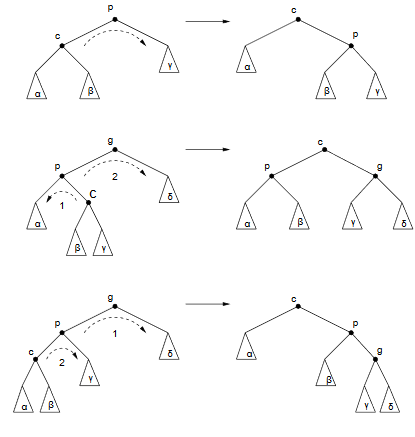
\includegraphics[width=0.5\textwidth]{splay_bottomup}
    \caption{Bottom-up splay.}
    \label{fig:splay_bottomup}
\end{figure}
\begin{itemize}
    \item De knoop wordt eerst gezocht zoals bij een gewone zoekboom.
    \item De splay-operatie gebeurt van onder naar boven.
    \item Een knoop kan naar boven gebracht worden door hem telkens te roteren met zijn ouder.
    \item Om de toegangstijd van knopen op de zoekweg ook te verbeteren, zijn er drie verschillende rotaties:
    \begin{enumerate}
        \item \textbf{De ouder $p$ van $c$ is wortel}. 
        \begin{itemize}
            \item Roteer beide knopen.
        \end{itemize}
        \item \textbf{Knoop $c$ heeft nog een grootouder}.
        \begin{itemize}
            \item Er zijn vier gevallen, die uitvallen in groepen van twee, naar gelang dat $p$ een linker- of rechterkind is van grootouder $g$.
            \item We veronderstellen dat $p$ linkerkind is van $g$.
        \end{itemize}
        
        \begin{enumerate}
            \item \textbf{Knoop $c$ is een rechterkind van $p$}.
            \item \textbf{Knoop $c$ is een linkerkind van $p$}.
        \end{enumerate}
    \end{enumerate}
\end{itemize}
\subsection{Top-down splayboom}


\section{Gerandomiseerde zoekbomen}
\label{sec:gerandomiseerde-zoekbomen}